%============================================================
\section{Nombre: Disparo de tonalli.}\label{hab.disparoT}
\subsection{Descripción}
Con ayuda de la caracola permite a su portador disparar tonalli. El disparo, al hacer contacto con el enemigo, reducirá la cantidad de vida de éste en caso de ser un jefe o lo destruirá en caso de ser un enemigo normal. Si el disparo colisiona con cualquier objeto, enemigo, ítem u obstáculo que no sea el jugador, el disparo se destruirá sin afectar el objeto, enemigo, ítem u obstáculo con el que haya colisionado. El disparo se destruirá si después de un periodo de tiempo no ha colisionado con ningún objeto u enemigo.
\subsection{Portador}
Malinalli
\subsection{Esquema}
			Ver figura \ref{fig:disparoT}.
			\begin{figure}
				\centering
				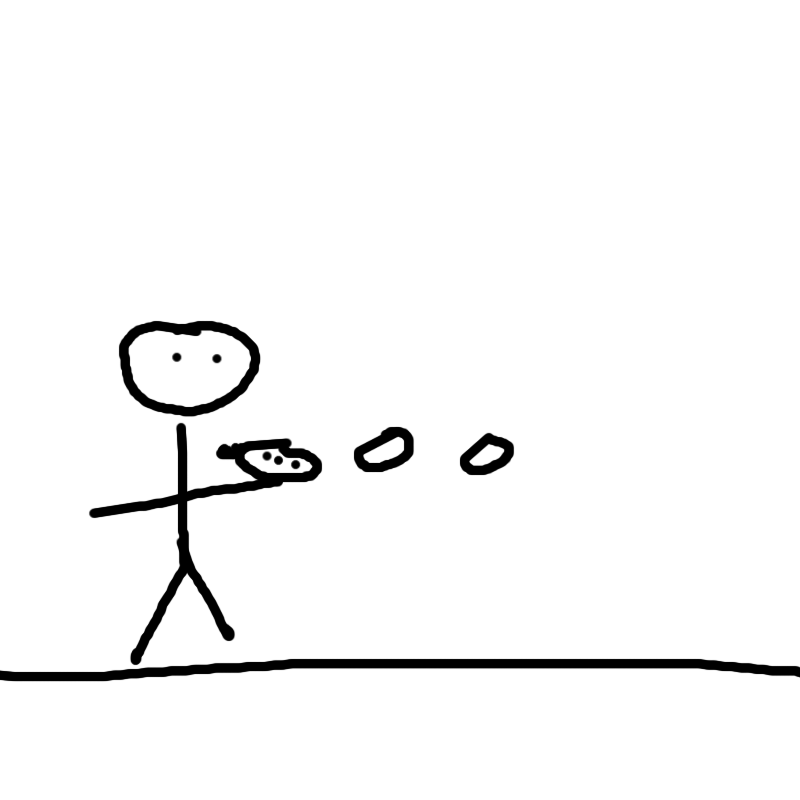
\includegraphics[height=0.2 \textheight]{Imagenes/disparoT}
				\caption{Disparo de tonalli por el jugador.}
				\label{fig:disparoT}
			\end{figure}